\chapter{Experimente und Ergebnisse}\label{ch:evaluation}

\section{Laufzeitverhalten}

Um das Laufzeitverhalten zu testen, wurden über einen Zeitraum von 30 Minuten eine Szene mit 412 Objektmengen mit insgesamt 2450 Objektposen aufgezeichnet.
Jede Objektmenge hatte dabei 6 Objekte, welche aus mehreren Objekterkennungssystemen stammten.

Das Testsystem bestand aus einem Intel$^\text{\textregistered}$ Core\texttrademark\ i5-750 Prozessor mit 2.67 GHz und 4 GiByte Hauptspeicher.
Als Betriebssystem wurde Ubuntu 12.04.03 LTS - Precise Pangolin mit dem Linux Kernel 3.2.0-52-generic-pae im 32 Bit Modus verwendet.
Die für den Testbetrieb verwendete SQLite-Datenbank wurde auf einer 100 Megabyte großen Ramdisk abgelegt, um Verzögerungen durch eine rotierende Festplatte zu vermeiden.

Die eigentlichen Tests wurden vollautomatisch durch den in Abschnitt \vref{impl:testrunner} vorgestellten \textbf{testRunner} durchgeführt.
In Tabelle \vref{tab:permutationen} sind sämtliche verwendeten Parameter aufgelistet.
Es wurden sämtliche Permutationen der dargestellten Parameter untersucht.

\begin{table}
\caption{Evaluationsparameter}
\label{tab:permutationen}
\begin{tabularx}{\textwidth}{ |l|X| }
 \hline
 Objektmengen & 50, 100, 150, 200, 250, 300, 350, 400 \\
 \hline
 Objekte pro Objektmenge & 2, 4, 6 \\
 \hline
 Bucketgröße & 0.5m, 0.3m, 0.1m, 0.09m, 0.07m, 0.05m, 0.03m, 0.01m \\
 \hline
 Benutze Clustering & Ja, Nein \\
 \hline
\end{tabularx}

\end{table}

Zu beachten ist, dass es sich bei Implicit Shape Models um ein reines Matching-Verfahren handelt, woraus folgt, dass nur Permutationen bereits gesehener Szenen erkannt werden können.
Aus diesem Grund ist es notwendig eine Vielzahl von Konstellationen über einen langen Zeitraum hinweg zu beobachten um eine möglichst breite Wissensbasis zu erhalten.
Diese Eigenart der ISMs hat auch zur Folge, dass alle durch das Modell mögliche Konstellationen sicher erkannt werden.
Daher war die Wiedererkennungsrate in allen Testdurchläufen nahe 100\%, weswegen in der Evaluation nicht näher auf die Erkennungsrate eingegangen wird.

\subsection{Ergebnisse}

\begin{figure}
  \centering
  \begin{subfigure}[b]{0.85\textwidth}
  \centering
  \includegraphics[width=1.0\textwidth]{bilder/eval1.pdf}
  \caption{Objektmengen und Objektzahlen.\\ Bucketgröße: 0.05m}
  \label{fig:eval-sc-oc}
  \end{subfigure}
  \begin{subfigure}[b]{0.85\textwidth}
  \centering
  \includegraphics[width=1.0\textwidth]{bilder/eval2.pdf}
  \caption{Bucketgrößen und Objektzahlen.\\ Objektmengen: 400}
  \label{fig:eval-bs-oc}
  \end{subfigure}
  \caption{Laufzeiten für unterschiedliche Objektmengenzahl, Objektzahlen, Bucketgrößen und Clustering}
\end{figure}

In Abbildung \vref{fig:eval-sc-oc} ist die Laufzeit unter Veränderung der Objektmengenanzahl dargestellt.
Die in der Legende aufgeführten Bezeichner "`NC"' und "`C"' stehen für "`Non-Clustered"' beziehungsweise "`Clustered"'.
Die Zahlenwerte repräsentieren jeweils die Anzahl der Objekte innerhalb jeder Objektmenge.
Erwartungsgemäß tritt deutlich hervor, dass die Laufzeit mit verwendetem Clustering und steigender Objektzahl deutlich höher ist als die Version ohne Clustering.
Dies ist durch die Wiederholung des Voting-Vorgangs in jeder Hierarchiestufe zu erklären.
In der gewählten Szene gab es jeweils zwischen zwei Objekten eine direktionale Beziehung, wodurch entsprechend $N-1$ Hierarchieebenen generiert wurden.
Zu beachten ist, dass dies dem Worst-Case-Verhalten einer statischen Szene entspricht.
In sehr dynamischen Szenen, in denen nur sehr wenige Objekte in Relation zueinander stehen, wird die Anzahl an Hierarchieebenen und damit auch ein signifikanter Teil der Laufzeit reduziert sein, was später in Abschnitt \vref{ch:eval-veränderlich} ersichtlich wird.
Hervorzuheben ist auch, dass trotz der großen Anzahl an Zusammenhängen und einer sehr hohen Zahl an Votes die längste Erkennungszeit für die Erkennung aller 6 Objekte mit aktiviertem Clustering nur 10ms betrug, womit eine Szenenerkennung mit einer Bildwiederholfrequenz gängiger Kameras problemlos möglich ist.

In Abbildung \vref{fig:eval-bs-oc} ist der Einfluss der Bucketgröße dargestellt.
Die Laufzeit ist auch hier überwiegend niedrig, wobei der rasante Anstieg der Laufzeit bei sehr niedrigen Bucketgrößen folgendermaßen zu erklären ist:\\
Die Ungenauigkeit der verwendeten Objekterkenner lag weit über $0.01m$, was zur Folge hatte, dass bei sehr kleinen Bucketgrößen sehr viele nur schwach befüllte Buckets existierten.
Da der komplette Einpassungsvorgang für jeden Bucket durchgeführt wird und das Verfahren es erlaubt sehr viele Votes innerhalb eines Buckets zu "`überspringen"', nachdem ein Vote eingepasst wurde.
Es ist bei vielen wenig befüllten Buckets jedoch weniger häufig möglich entsprechende Abkürzungen zu benutzen.
Daher steigt der Gesamtrechenaufwand stark an, wenn bei starkem Sensorrauschen und kleinen Bucketgrößen ein neuer Bucket für jedes Positionsabweichnug erstellt wird.

\section{Verhalten bei veränderlichen Szenen}\label{ch:eval-veränderlich}

\subsection{Versuchsaufbau}

Im zweiten Versuch wird eine typische Schreibtischszene aufgezeichnet.
Sie bestand aus zwei Monitoren, welche vor einer Tastatur und Maus angeordnet wurden.
Im Laufe der Aufzeichnung wurden Maus und Tastatur entsprechend ihrer normalen Benutzung bewegt sowie die Höhe der beiden Monitore verändert.
Eine Darstellung der aufgenommen Spuren der Szenenkomponenten ist in Abbildung \vref{fig:schreibtisch-record} ersichtlich.

\begin{figure}
  \centering
  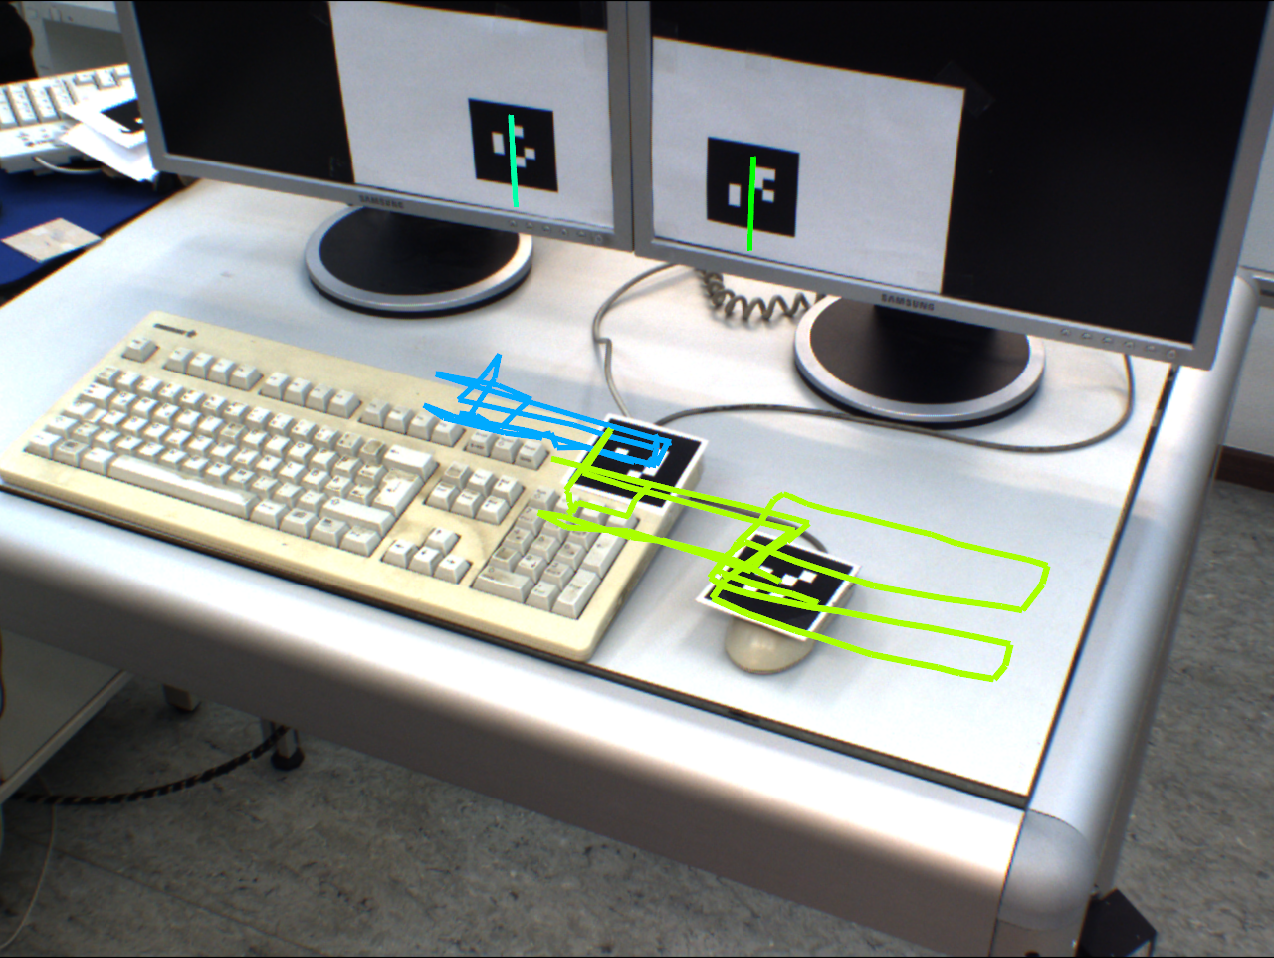
\includegraphics[width=0.7\linewidth]{bilder/paper_fotos/training-data-camera.png}
  \caption{Versuchsaufbau der Schreibtischszene mit eingezeichneten Spuren der beteiligten Objekte. Bildquelle: \cite{P.MeissnerandR.RecklingandR.JaekelandS.R.Schmidt-RohrandR.Dillmann2013}}
  \label{fig:schreibtisch-record}
\end{figure}

\subsection{Modellbildung}

Abbildung \vref{fig:schreibtisch-record-data} zeigt deutlich, dass das generierte Modell korrekte Cluster bildet.
Die Heuristik hat die beiden Monitore in eine Unterszene zusammengefasst, zudem wurden die Maus und Tastatur ebenfalls zueinander in Beziehung gesetzt.
Erkennbar ist dies durch die gezeichneten Votingvektoren.
Zu beachten ist dass die eingezeichneten Vektoren jeweils vom Referenzpunkt der Unterszene auf die verbundenen Objekte zeigen.
Daran ist zu sehen, das die Votes des linken Monitors nur vom rechten Monitor abhängen, was bedeutet dass der rechte Monitor als Referenzobjekt in der Unterszene ausgewählt wurde.
Analog ist die Maus nur durch die Tastatur mit dem Modell verbunden.
Die beiden Unterszenen sind wiederum durch Votes hin zur Tastatur, ausgehend vom rechten Monitor verbunden.
Es ist wichtig zu erwähnen dass dies nicht bedeutet, dass die Szene bei fehlendem rechten Monitor nur mit 50\% Konfidenz erkannt wird:\\
Entsprechend dem Erkennungsalgorithmus wird aus den Votes des linken Monitors bei fehlendem rechten Monitor ein virtuelles Objekt für die Unterszene generiert, welches an der erwarteten Position des rechten Monitors platziert wird.
Dieses generierte Objekt besitzt aufgrund des Fehlens des rechten Monitors jedoch nur das Gewicht 1, woraus eine Gesamtkonfidenz der Szenenerkennung für die erkannte Szene von 75\% resultiert.

\begin{figure}
  \centering
  \includegraphics[width=0.7\linewidth]{bilder/paper_fotos/training-data.png}
  \caption{Versuchsaufbau der Schreibtischszene mit eingezeichneten Spuren und Votingvektoren der beteiligten Objekte. Bildquelle: \cite{P.MeissnerandR.RecklingandR.JaekelandS.R.Schmidt-RohrandR.Dillmann2013}}
  \label{fig:schreibtisch-record-data}
\end{figure}

\subsection{Erkennungsverhalten und Konfidenz}

\begin{figure}
 \begin{center}
  \begin{subfigure}[b]{.3\textwidth}
    \includegraphics[width=1\linewidth]{bilder/paper_fotos/s1.png}
  \end{subfigure}
  \begin{subfigure}[b]{.3\textwidth}
    \includegraphics[width=1\linewidth]{bilder/paper_fotos/s2.png}
  \end{subfigure}
  \begin{subfigure}[b]{.3\textwidth}
    \includegraphics[width=1\linewidth]{bilder/paper_fotos/s3.png}
  \end{subfigure}
  \begin{subfigure}[b]{.3\textwidth}
    \includegraphics[width=1\linewidth]{bilder/paper_fotos/s7.png}
  \end{subfigure}
  \begin{subfigure}[b]{.3\textwidth}
    \includegraphics[width=1\linewidth]{bilder/paper_fotos/s5.png}
  \end{subfigure}
  \begin{subfigure}[b]{.3\textwidth}
    \includegraphics[width=1\linewidth]{bilder/paper_fotos/s4.png}
  \end{subfigure}
  \begin{subfigure}[b]{.3\textwidth}
    \includegraphics[width=1\linewidth]{bilder/paper_fotos/s6.png}
  \end{subfigure}
  \begin{subfigure}[b]{.3\textwidth}
    \includegraphics[width=1\linewidth]{bilder/paper_fotos/s8.png}
  \end{subfigure}
  \begin{subfigure}[b]{.3\textwidth}
    \includegraphics[width=1\linewidth]{bilder/paper_fotos/s9.png}
  \end{subfigure}
  \begin{subfigure}[b]{.3\textwidth}
    \includegraphics[width=1\linewidth]{bilder/paper_fotos/s10.png}
  \end{subfigure}
  \begin{subfigure}[b]{.3\textwidth}
    \includegraphics[width=1\linewidth]{bilder/paper_fotos/s11.png}
  \end{subfigure}
  \begin{subfigure}[b]{.3\textwidth}
    \includegraphics[width=1\linewidth]{bilder/paper_fotos/s12.png}
  \end{subfigure}
  \begin{subfigure}[b]{.3\textwidth}
    \includegraphics[width=1\linewidth]{bilder/paper_fotos/s13.png}
  \end{subfigure}
  \begin{subfigure}[b]{.3\textwidth}
    \includegraphics[width=1\linewidth]{bilder/paper_fotos/s15.png}
  \end{subfigure}
  \caption{Erkennungsergebnisse für unterschiedliche Objektkonfigurationen. Bildquelle: \cite{P.MeissnerandR.RecklingandR.JaekelandS.R.Schmidt-RohrandR.Dillmann2013}}
  \label{fig:schreibtisch-konfigurationen}
 \end{center}
\end{figure}

In Abbildung \vref{fig:schreibtisch-konfigurationen} ist eine Serie von Konfigurationsänderungen abgebildet.
Die Elemente der Visualisierung wurden bereits in Abschnitt \vref{impl:visualisierung} näher erläutert.
Im Folgenden werden die einzelnen Szenenänderungen erklärt und verdeutlicht, warum das beobachtete Verhalten dem gewünschten Verhalten entspricht.

Das erste Bild enthält eine normale erfolgreiche Erkennung der Ausgangskonfiguration der Objekte, die grünen Linien sind ein Indikator für eine Erkennungskonfidenz von 100\%.
Im zweiten Bild wurde der rechte Monitor nach unten verschoben, daraus ergibt sich eine unvollständige Szene.
Anhand der roten Linie der Unterszene zwischen den beiden Monitoren ist zu erkennen, dass die Konfidenz der Unterszene auf $\leq$50\% gefallen ist, was zu erwarten ist, da einer von zwei Monitoren eine nonkonforme Position eingenommen hat.
Die grüne Linie zwischen Maus und Tastatur stellt eine vollständige Unterszene dar.
Die orange Linie zwischen den beiden Teilszenen spiegelt eine Gesamtkonfidenz der Szene von 75\% wider.
Dies entspricht den erwarteten Ergebnissen.

Das dritte Bild zeigt den rechten Monitor an der richtigen Position, jedoch mit einer nonkonformen Orientierung relativ zu den anderen Objekten.
Abermals wird der rechte Monitor aus dem Modell ausgeschlossen und die Szene erhält eine Erkennungskonfidenz von 75\%.
Ein analoges Ergebnis liefern die horizontalen Verschiebungen in Bild 4 und 5.

Die Bilder 6 und 7 zeigen entsprechende Ergebnisse für das Verschieben und Drehen des linken Monitors.

In den Bildern 8 und 9 sind jeweils valide Mausbewegungen erkennbar, welche den erwarteten Positionen des Modells entsprechen und zu einem Erkennungsergebnis von 100\% führen.

Bild 10 zeigt die Maus, welche um 90$^\circ$ gedreht wurde.
Diese wird, wie erwartet, als nicht der Szene zugehörig erkannt.
Das Gleiche gilt auch für Bild 11 in dem die Maus vor die Tastatur platziert worden ist.

In Bild 12 wurde die Tastatur gedreht, wodurch von der Maus ausgehend ein virtuelles Objekt für die nicht passende Tastatur gebildet wird.
Das geschieht, weil für jeden Referenzpunkt einer Teilszene, ob vollständig oder nicht, ein Objekt in die Eingabemenge eingefügt wird, um diese Teilszene als ein Objekt in der Hierarchie zu vertreten.
Da der Algorithmus die vorhandenen Votes im Rahmen der gesetzten Grenzwerte in die Szene einpasst, auch wenn sie nicht perfekt passen oder besser passendes Votes existieren, ist zu erkennen, dass die von der Maus ausgehende Unterszene die Monitor-Unterszene mit einer gewissen Abweichung "`trifft"'.
Da dies jedoch durch die entsprechende Bucketgröße explizit erlaubt ist, beträgt das Gesamtergebnis wie erwartet 75\%.
Eine ähnliche Situation ist auch in Bild 13 gegeben, in der die Tastatur seitlich verschoben wurde.

Das letzte Bild zeigt die Maus, wie sie im Raum über der Tastatur hängt, wodurch sie erwartungsgemäß von dem Erkenner ignoriert wird.
Es ergibt sich die erwartete Konfidenz von 75\%.
